\begin{frame}

\frametitle{Model-based economic evaluation}

\bi

\item Trial-based economic evaluation
  \begin{itemize}
  \item assess cost-effectiveness based on individual-level data on
    costs and effects
  \item shorter-term, selected population
  \end{itemize}

\item Model-based economic evaluation
  \begin{itemize}
  \item construct a model-based representation of disease/clinical
    history
  \item State-transition (usually \emph{Markov}) models for clinical
  histories very common
  \item ``populate'' model with available + relevant data.
  \end{itemize}

\item Model-based evaluation typically used to estimate
  \begin{itemize}
  \item \alert{long-term} cost-effectiveness
  \item in wider population 
  \end{itemize}
  by combining data from trials with other sources of evidence.

\ei

\vfill 
\begin{block}{\footnotesize References}
\bmhe,  chapter 5.4.\\
\esdmh
\end{block}
\end{frame}

%### New page ############################################################

\frame{%
\frametitle{Summary}
\begin{itemize}
\item Decision tree model
\begin{itemize}
\item Strengths and limitations
\item When to use and when not use
\end{itemize}
\item How to calculate on a decision tree
\begin{itemize}
\item `Forward' method
\item `Backward' method
\end{itemize}
\item Examples
\end{itemize}

\vfill
\begin{block}{\footnotesize References}
Decision Making in Health and Medicine, Weinstein et al, Cambridge University Press
\end{block}

}


\begin{frame}
\frametitle{Steps in constructing and analysing Decision Trees}
A decision tree is a visual representation of a decision analysis:
	\begin{itemize}
		\item \alert{Structure} the tree
		\pause
		\item Estimate \alert{probabilities}
		\pause
		\item Estimate \alert{payoffs} (assign values to costs and outcomes)
		\pause
		\item Analyse the tree
		\pause
			\begin{itemize}
				\item \alert{Evaluate} the tree
				\item Explore \alert{uncertainty}
			\end{itemize}
	\end{itemize}
\end{frame}

\begin{frame}
\frametitle{Structuring the Decision Tree}
A decision tree is made up of nodes, branches and outcomes

\begin{itemize}
	\item Nodes:
	\begin{itemize}
		\pause
		\item \textcolor{blue}{Decision node (square)}: Describes the problem. Deterministic choice.
		\pause
		\item \textcolor{green}{Chance node (circle)}: Represents the point at which several possible events can occur.
		\pause
		\item \textcolor{red}{Terminal node (triangle)}: Represents the end of a tree with a payoff attached.
	\end{itemize}
\end{itemize}
\end{frame}

\begin{frame}
A hypothetical example is of a comparison between two drugs, `Drug A' and
`Drug B'. Each drug has different costs associated with them and
different performance in terms of the chance that the drug is successful at treating the patient.

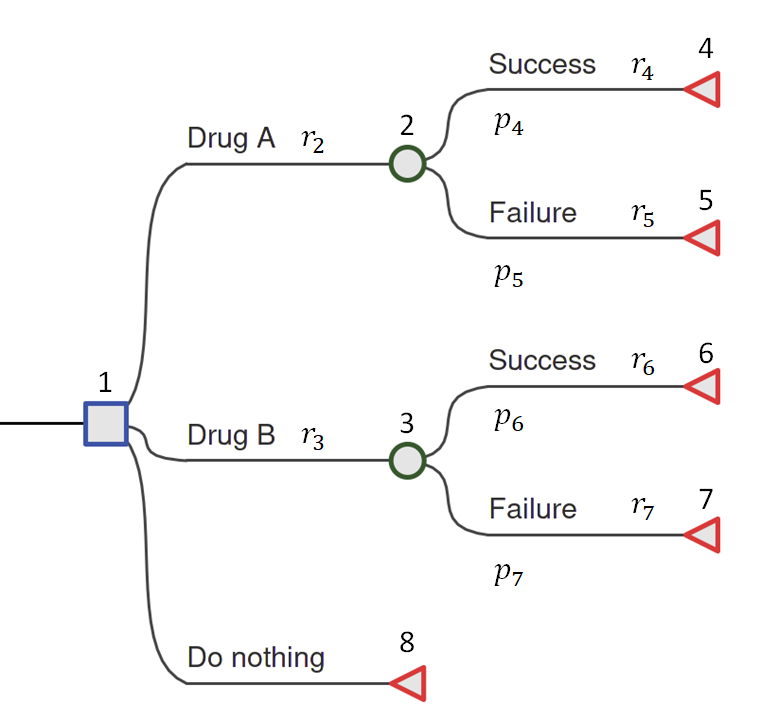
\includegraphics[width=\textwidth,height=0.8\textheight, keepaspectratio]{decision-trees/figs/dectree.png}

\end{frame}

\begin{frame}
\frametitle{Structuring the Decision Tree}
	\begin{itemize}
		\item Branches issuing from a chance node represent possible events patients may experience at that point in the tree.
		\item Branch probabilities represent the likelihood of each event.
		\item The sequence of chance nodes from left to right usually follows the sequence of events.
		\item The events stemming from a chance node must be \alert{mutually exclusive} and probabilities should sum to 1.
	\end{itemize}
\end{frame}


\begin{frame}
\frametitle{Advantages of Decision Trees}

	\begin{itemize}
		\item They enable the economic question to be structured in a \alert{meaningful} and \alert{visual} manner.
		\pause
		\item  They allow data informing the model parameters to be assimilated and, where appropriate, synthesised.
		\pause
		\item They are relatively simple to undertake and suitable for:
		\begin{itemize}
			\item Diseases that occur only once.
			\item Decisions about acute care.
			\item Decisions with short time frames.
		\end{itemize}
	\end{itemize}
\end{frame}


\begin{frame}
\frametitle{Limitations of Decision Trees}

	\begin{itemize}
		\item They do not explicitly account for passage of time:
			\begin{itemize}
				\item Passage of time accounted for by outcome measure.
				\item Limited ability to account for long term outcomes.
			\end{itemize}
			\pause
		\item Possible to add branches but results in a complex model.
		\item Other modelling techniques can handle repeated events better.
		\item Structure of tree only allows for one-way progression of patient through model: Not movement back and forth between states.
		\item Decision trees can still be useful as a sub-model.
		\end{itemize}
\end{frame}


\begin{frame}
\frametitle{}
 
\includegraphics[width=1\textwidth,height=1.2\textheight, keepaspectratio]{decision-trees/figs/nice-guidance}
\end{frame} 

\begin{frame}
\frametitle{Simple decision tree example: New TST guidelines}
 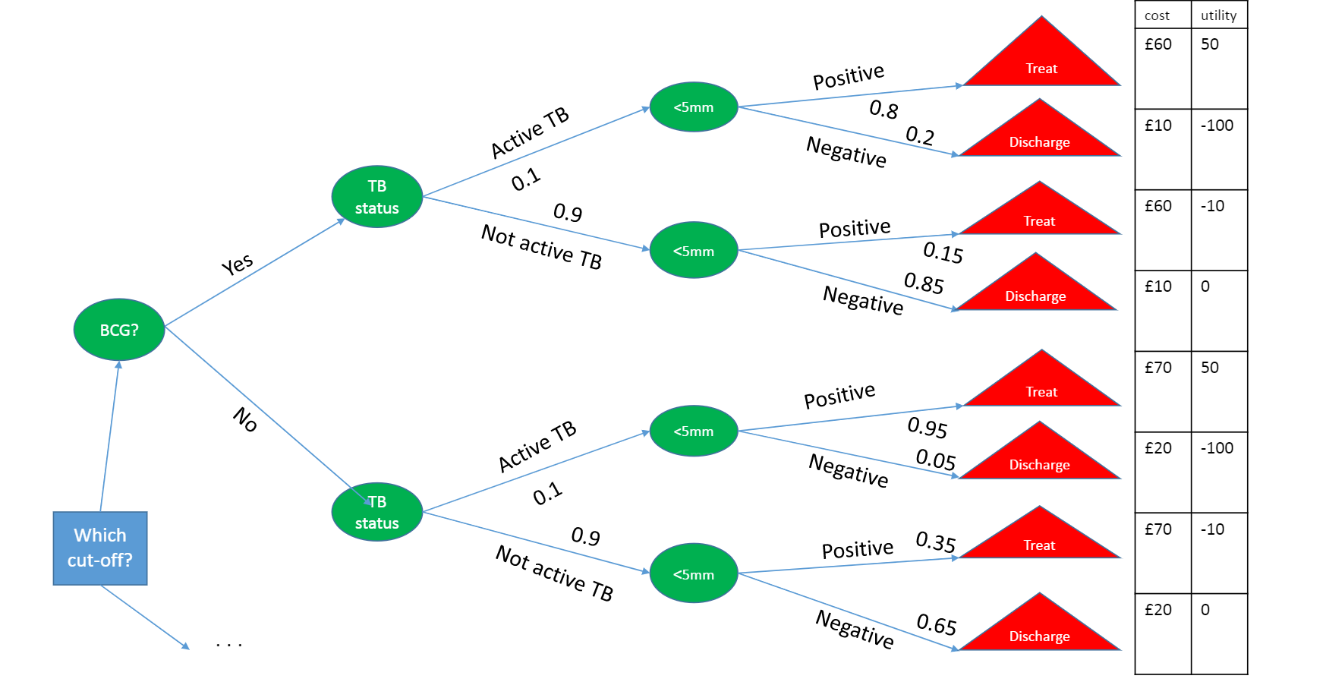
\includegraphics[width=\textwidth,height=0.8\textheight, keepaspectratio]{decision-trees/figs/tb-decision-tree}
\end{frame}


\begin{frame}
\frametitle{Calculations on a decision tree}

\begin{itemize}
 \item Conditional probabilities two or more events 
 \item Probability of both A and B occurring, divided by the probability of B occurring
 \item The joint probability of A and B measures the probability that A and B occur together at the same moment.
 \item The marginal probability of A is the individual probability of A, ignoring any value of event B.
\end{itemize}

\end{frame}

\begin{frame}
\frametitle{Probabilities of moving along branches}

\begin{itemize}
 \item Complete set of all possible outcomes is set of terminal nodes on the RHS
\pause
 \item By chaining the conditional probabilities for a given pathway we obtain the total or
\emph{joint} probability of reaching a terminal node. Each pathway
through the tree is a mutually exclusive sequence of events. Consider
one such pathway through the tree with the following \(n\) nodes.

\[
x_0 \rightarrow x_{[1]} \rightarrow x_{[2]} \rightarrow \cdots \rightarrow x_{[n]}
\]
where 
\begin{itemize}
\item \(x_0\) is the root node (often the decision node)
\item \(x_{[n]}\) is the terminal node and the square brackets indicate that this is the \(ith\) ordered nodes in the sequence.
\end{itemize}
\pause
 \item By the product rule joint probability of this path is

\[
p(x_{[1]}, x_{[2]}, \ldots, x_{[n]}) =
p(x_{[2]} \mid x_{[1]}) p(x_{[3]} \mid x_{[2]}) \cdots  p(x_{[n]} \mid x_{[n - 1]}) =
\]
\[
\prod_i^{[n - 1]} p(x_{[i + 1]} \mid x_{[i]})
\]
\pause
 \item For the above pathway, the corresponding cost and effects are
\(c_{[1]}, c_{[2]}, \ldots, c_{[n]}\) and
\(e_{[1]}, e_{[2]}, \ldots, e_{[n]}\).
\end{itemize}

\end{frame}

\begin{frame}
\frametitle{How to calculate expected values}

There are two alternative approaches used for calculating the expected
cost and effectiveness on a decision tree.

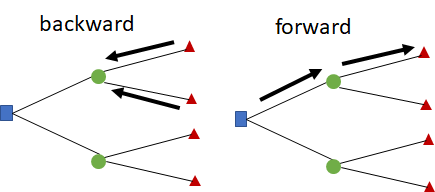
\includegraphics{decision-trees/figs/forward-backward-diagram.png}

\end{frame}

\begin{frame}
\frametitle{"Backward" computation}

\begin{itemize}
 \item Weighted average of the total values of the child nodes of a parent chance node
 \begin{itemize}
  \item Weights are the probability of traversing each branch to the child nodes.
 \end{itemize}
\pause
 \item Act of stepping backwards in this way through the tree is called \emph{folding back} (or \emph{rolling back}).
\pause
 \item So called because the children are folded up or collapsed, so that the chance node is now represented by its expected value.
\pause
 \item Starting at the right-most terminal nodes the expected values at each chance node are calculate in turn and the tree can thus be folded back all the way to the decision node
\pause
 \item Example of something called a \emph{recursive} function which is a function that calls itself during its execution.
 \begin{itemize}
  \item A well-known example is when calculating the Fibonacci series.
  \end{itemize}
 \item This approach is part of a whole field of stochastic optimisation in applied probability called Markov decision process (MDP).
 \end{itemize}

\end{frame}

\begin{frame}
\frametitle{"Backward" computation}

\begin{itemize}
 \item Recall the conditional probabilities \(p_{ij} = p(x_j \mid x_i)\), then
the expected value is

\[
\mathbb{E}[V_i] =   \left\{
    \begin{array}{lcl}
      r_i & \mbox{ if } & i \in \mathcal{S}_{term}\\
      r_i + \sum p_{ij} \mathbb{E}[V_j] & & \mbox{otherwise}
    \end{array}
  \right.
\]
where
\begin{itemize}
\item \(\mathbb{E}\) is the weighted average of the values, \(V\) is the random variable total node value, e.g.~cost or QALYs
 \item \(r_i\) is the (unit) value at node \(i\)
 \item \(\mathcal{S}_{term}\) is the set of all terminal nodes. Note that at a terminal node the expected value is simply the value at that node.
\pause
 \end{itemize}
 \item An advantage of using this method is that total expected values can be obtained at each node and so if there are multiple decision node not at the root of the tree the recursive approach can fold-back sub-trees.
\end{itemize}

\end{frame}

\begin{frame}
\frametitle{Simple decision tree example: New TST guidelines}
 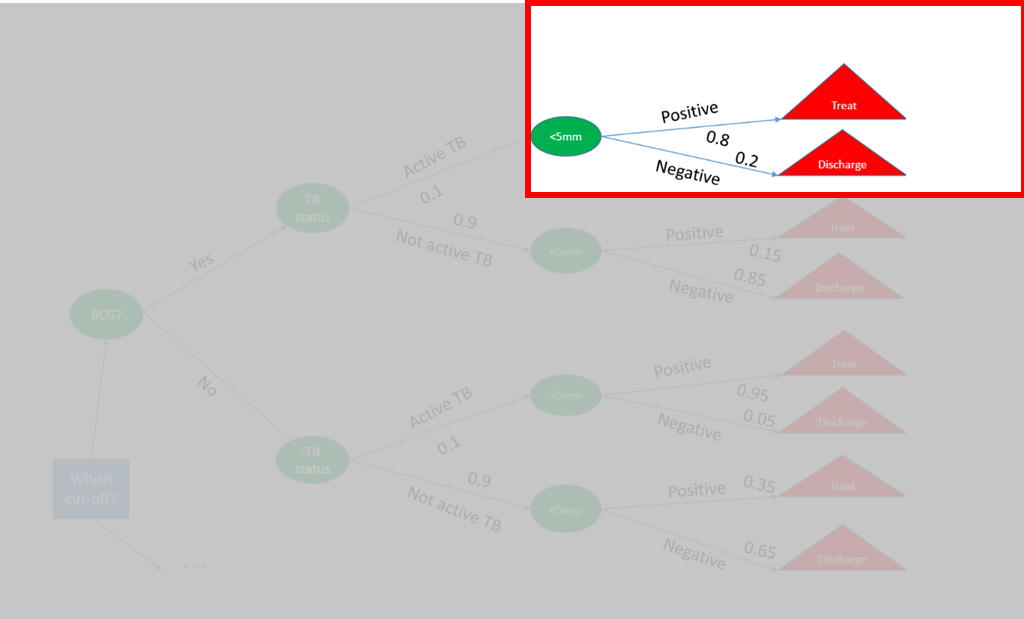
\includegraphics[width=\textwidth,height=0.8\textheight, keepaspectratio]{decision-trees/figs/folding-back1}
\end{frame}

\begin{frame}
\frametitle{Simple decision tree example: New TST guidelines}
 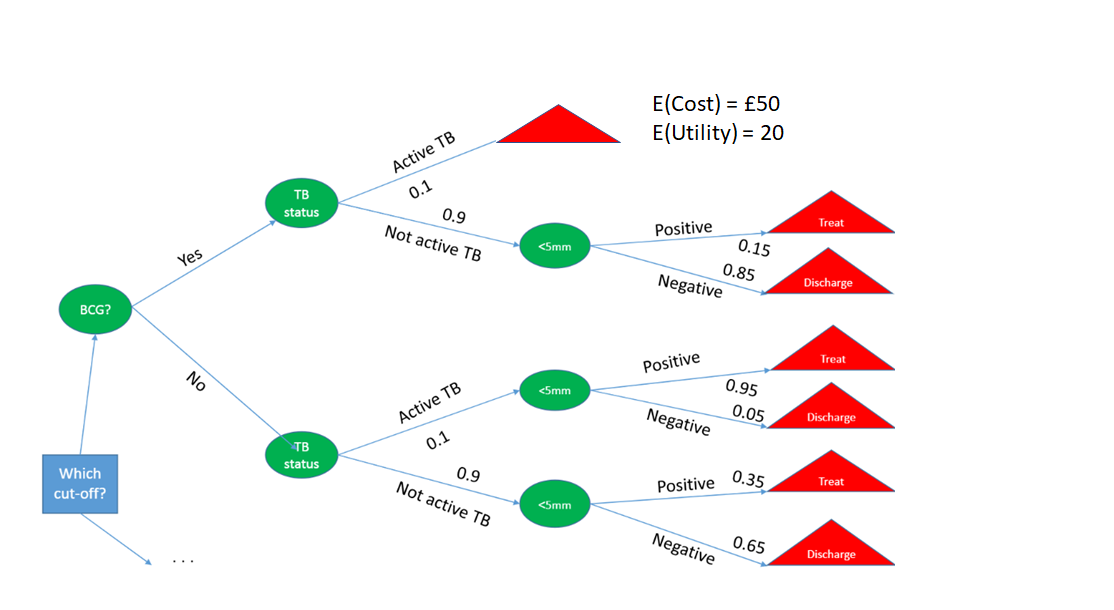
\includegraphics[width=\textwidth,height=0.8\textheight, keepaspectratio]{decision-trees/figs/folding-back2}
\end{frame}

\begin{frame}
\frametitle{Simple decision tree example: New TST guidelines}
 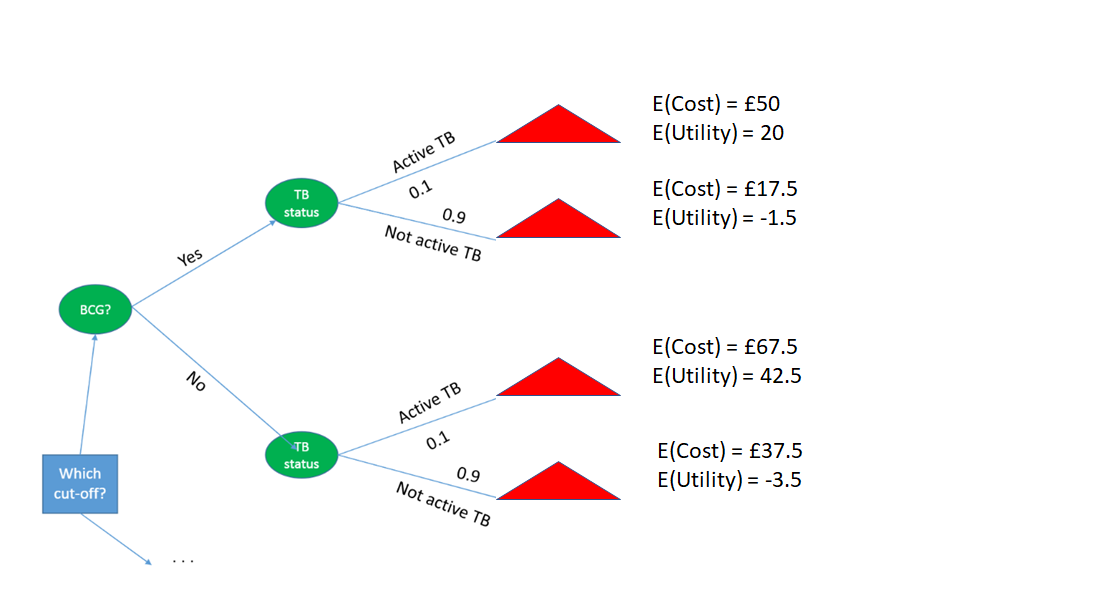
\includegraphics[width=\textwidth,height=0.8\textheight, keepaspectratio]{decision-trees/figs/folding-back3}
\end{frame}

\begin{frame}
\frametitle{Simple decision tree example: New TST guidelines}
 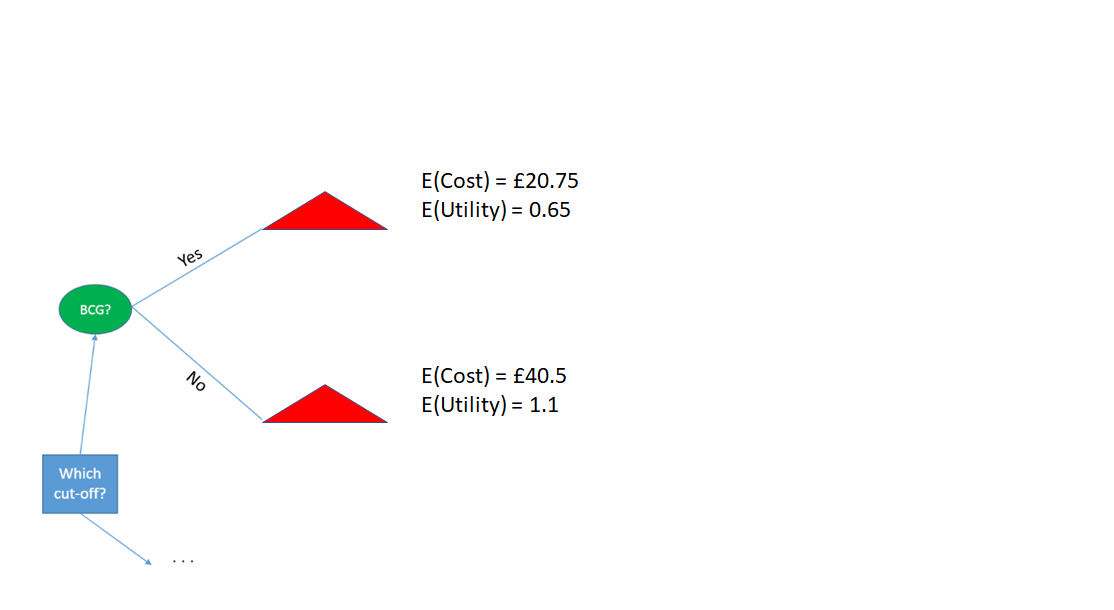
\includegraphics[width=\textwidth,height=0.8\textheight, keepaspectratio]{decision-trees/figs/folding-back4}
\end{frame}


\begin{frame}
\frametitle{"Forward" computation}

 \begin{itemize}
 \item May be more intuitive
\pause
 \item Calculate the total health and costs, and joint probability along all of the distinct pathways of the tree corresponding to a decision.
\pause
 \item The weighted average of the costs or health values give the expected value at the decision node.
\pause

\item Formally

\[
\mathbb{E}[V] = \sum_{j \in S_{term}} r^*_j p^*_j
\]
where

 \begin{itemize}
 \item \(r^*_j = r_{[1]} + r_{[2]} + \cdots + r_{[n]}\) is the total of the values along each pathway with terminal node \(j\)
 \item \(p^*_j = p(x_{[1]}, x_{[2]}, \ldots, x_{[n]})\) is the joint probabilities of traversing the unique path with terminal node \(j\).
 \item The set of possible terminal nodes if the decision-maker takes a given decision is denoted \(S_{term}.\)
 \end{itemize}
\end{itemize}

\end{frame}


\begin{frame}
\frametitle{TB Combined probabilities for each branch}
 If probability of BCG is $0.1$ (c.f. NHS Immunisation Statistics, England 2012-13) then
\begin{eqnarray*}
p^*_1 &=& 0.1 \times 0.1 \times 0.8 = 0.008\\
p^*_2 &=& 0.1 \times 0.1 \times 0.2 = 0.002\\
p^*_3 &=& 0.1 \times 0.9 \times 0.15 = 0.0135\\
p^*_4 &=& 0.1 \times 0.9 \times 0.85 = 0.0765\\
p^*_5 &=& 0.9 \times 0.1 \times 0.95 = 0.0855\\
p^*_6 &=& 0.9 \times 0.1 \times 0.05 = 0.0045\\
p^*_7 &=& 0.9 \times 0.9 \times 0.35 = 0.2835\\
p^*_8 &=& 0.9 \times 0.9 \times 0.65 = 0.5265
\end{eqnarray*}
\end{frame}

\begin{frame}
\frametitle{TB expected cost and health impact}

Cost:

\begin{eqnarray*}
&& 0.008 \times 60 + 0.003 \times 10 + 0.0135 \times 60 + 0.0765 \times 10\\
&& + 0.0855 \times 70 + 0.0045 \times 20 + 0.2835 \times 70 + 0.5265 \times 20\\
&& = 38.535
\end{eqnarray*}

Health:

\begin{eqnarray*}
&& 0.008 \times 50 + 0.003 \times (-100) + 0.0135 \times (-10) + 0.0765 \times 0\\
&&  + 0.0855 \times 50 + 0.0045 \times (-100) + 0.2835 \times (-10) + 0.5265 \times 0\\
&& = 0.955
\end{eqnarray*}

\end{frame}

\begin{frame}
\frametitle{Decision tree practical}
 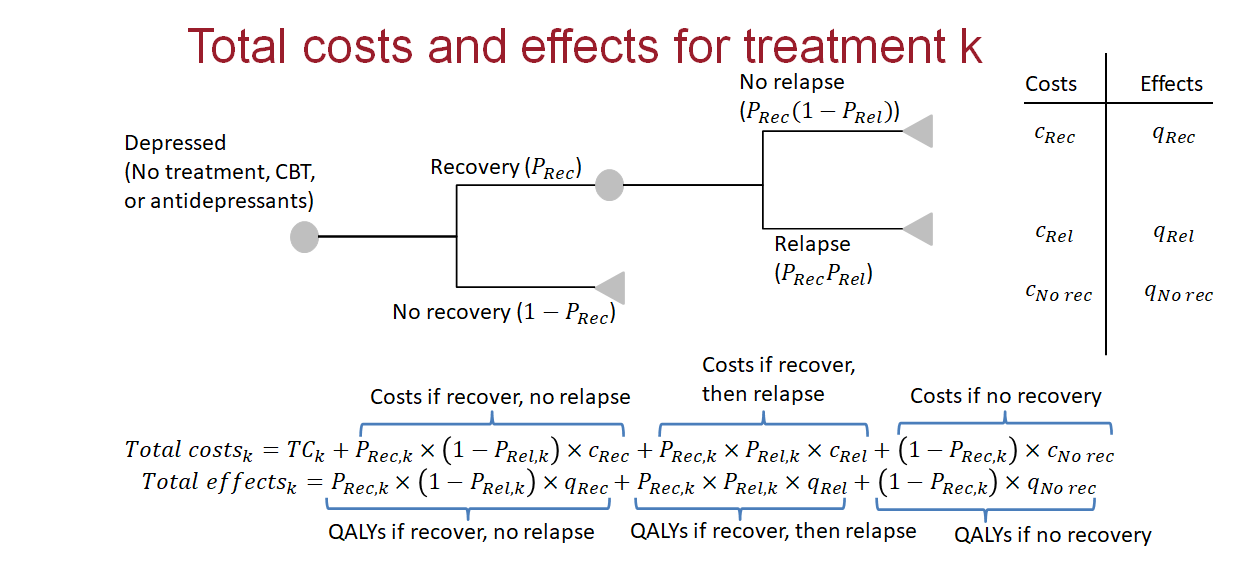
\includegraphics[width=\textwidth,height=0.8\textheight, keepaspectratio]{decision-trees/figs/practical-decision-tree}
\end{frame}



